\chapter{Discussion}
\label{cha:discussion}

% \section{Evaluation}
% \label{sec:evaluation}
\begin{comment}

When evaluating your results, avoid drawing grand conclusions, beyond those that your results can in fact support.
Further, although you may have designed your experiments to answer certain questions,
the results may raise other questions in the eyes of the reader.
It is important that you study the graphs/tables to look for unusual features/entries, and discuss these as well as the main findings.
In particular, carry out an error analysis: What went wrong and why?

A confusion matrix can, for example, be a good way to display misclassifications.
Figure~\ref{fig:conf_sentiment} (on Page~\pageref{fig:conf_sentiment}) shows two confusion matrices.
If there were perfect correlation between true and predicted labels, the long diagonals (from the upper left to the lower right corner) would be completely red.
However,  the confusion matrices indicate
that this classifier was quite biased towards the neutral label (illustrated with \Neutrey),
as can be seen from the warm colours in the positive (\Smiley) and negative (\Sadey) true label cells of the \Neutrey predicted label column.

% Axis configuration for confusion matrices with pgfplots
\pgfplotsset{
    colormap={whitehot}{color(0cm)=(white); color(1cm)=(yellow); color(2cm)=(orange); color(3cm)=(red)},
    confusionaxis/.style={
            colorbar,
            colorbar style={
                    width=2mm,
                    at={(1.05,1)},
                },
            colormap name=whitehot,
            faceted color=none, % remove lines between fields
            view={0}{90},
            y dir=reverse,
            xlabel=Predicted label,
            ylabel=True label,
            tick style={draw=none},
            yticklabels={,,},
            xticklabels={,,},
            every node=[font=\small],
            extra x ticks={0.4,1.5,2.6},
            extra x tick labels={\Smiley, \Neutrey, \Sadey},
            extra y ticks={0.3,1.5,2.7},
            extra y tick labels={\Smiley, \Neutrey, \Sadey},
            extra x tick style={
                    x tick label style={
                            font=\Large
                        }
                },
            extra y tick style={
                    y tick label style={
                            font=\Large
                        }
                },
            width=.4\linewidth,
        }
}

\begin{figure}[t!]
    \centering
    \begin{subfigure}{\linewidth}
        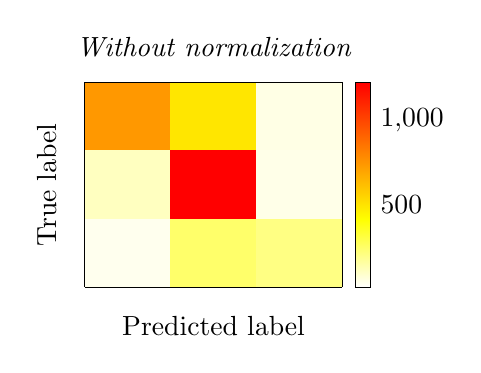
\begin{tikzpicture}
            \begin{axis}[
                    confusionaxis,
                    title={\em Without normalization},
                ]
                \addplot3
                [surf,mesh/cols=4,shader=flat corner
                ] coordinates {
                        (0,0,740) (1,0,490 ) (2,0,43 ) (3,0,1)
                        (0,1,102) (1,1,1229) (2,1,38 ) (3,1,1)
                        (0,2,28 ) (1,2,240 ) (2,2,199) (3,2,1)
                        (0,3,1  ) (1,3,1   ) (2,3,1  ) (3,3,1)
                    };
            \end{axis}
        \end{tikzpicture}
        %\hfill
        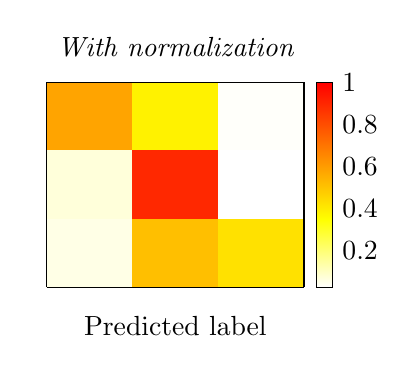
\begin{tikzpicture}
            \begin{axis}[
                    confusionaxis,
                    title={\em With normalization},
                    ylabel={},
                    colorbar style={
                            ylabel={},
                            yticklabel style={
                                    align=right,
                                }
                        },
                ]
                \addplot3
                [surf,mesh/cols=4,shader=flat corner
                ] coordinates {
                        (0,0,0.58130401) (1,0,0.38491752) (2,0,0.03377848) (3,0,1)
                        (0,1,0.07450694) (1,1,0.89773557) (2,1,0.02775749) (3,1,1)
                        (0,2,0.05995717) (1,2,0.51391863) (2,2,0.4261242 ) (3,2,1)
                        (0,3,1         ) (1,3,1         ) (2,3,1         ) (3,3,1)
                    };
            \end{axis}
        \end{tikzpicture}
        \label{fig:conf_sentiment_2013}
    \end{subfigure}
    \caption{Sentiment classifier confusion matrices}
    \label{fig:conf_sentiment}
\end{figure}

\end{comment}
% \section{Discussion}
% \label{sec:discussion}
\begin{comment}

In this section it is important to include a discussion of not just the merits of the work conducted, but also the limitations.
Which choices did you make? Why? What alternatives were there?
{\color{red}\textbf{Note that a key part of the Master's Thesis grading is based on the student's ability to discuss the results in light of the work by others as well as the restrictions and potential of the work itself.}}
While the Results section will report the outcome of each specific experiments, the Discussion should put those results into perspective and look at overall lessons that can be learned from the entire series of experiments.

You should be able to discuss your work in relation to its overall goal and your research questions (i.e., those introduced in Chapter~\ref{cha:introduction}),
but also address issues such as any ethical considerations that the work may entail,
as well as its technical challenges and limitations.

Discussion and evaluation can either be two different chapters, a joint chapter (as here), or part of the concluding chapter
--- or the discussion can be part of that chapter while the evaluation is part of the experimental chapter.

As for most parts of the thesis, it is possible to select various outlines and setups for the discussion; the important thing is that all the relevant parts appear \textit{somewhere\/} in the text.
\end{comment}

\Autosectionref{sec:geogpt-in-gis} will open the \nameref{cha:discussion} chapter by suggesting a place for an application like GeoGPT in the field of \acrshort{acr:gis}. Thereafter, \autoref{sec:why-sql-better} will present possible reasons as to why the \acrshort{acr:sql} agent outperforms the other two agent types. \Autosectionref{sec:autonomous-gis-struggles} will discuss problem encountered during the development of GeoGPT. Finally, \autoref{sec:multi-agent-architectures} will discuss a semi-failed attempt at implementing a multi-agent architecture for GeoGPT, and provide suggestions as to why this didn't succeed.

% \Autosubsectionref{subsec:dead-ends} will explore the scenarios in which GeoGPT repeatedly encounters dead ends, attempting the same unsuccessful actions multiple times. \Autosubsectionref{subsec:self-verification} will discuss how one of the autonomous goal of \textit{self-verification} --- introduced by \cite{liAutonomousGISNextgeneration2023} --- can be improved, for instance by utilizing the multi-modal abilities of certain state-of-the-art \acrshortpl{acr:llm}. 


\section[GeoGPT's Place in the Field of GIS]{GeoGPT's Place in the Field of \acrshort{acr:gis}}
\label{sec:geogpt-in-gis}

As stated in the section on \nameref{sec:goals-and-research-questions}, one of the goals of this thesis is to see if \acrshort{acr:llm}-based systems can replace \acrshort{acr:gis} professionals. Results from experiments comparing prompts designed to emulate expert and novice users, as detailed in \autoref{subsec:prompt-quality-test-results}, indicate that the role of \acrshort{acr:gis} professionals is not immediately threatened. As \autoref{fig:novice-vs-expert-munkegata-trees} shows, expert-level prompting is highly necessary to make GeoGPT consistently produce the desired outcomes for more complex tasks.

It is, however, clear that \acrshort{acr:llm} technologies have significant potential to automate tasks that \acrshort{acr:gis} professionals are commonly faced with. GeoGPT can therefore serve as a helpful companion --- much like GitHub Copilot\footnote{\url{https://github.com/features/copilot}} for software developers --- that can quickly solve a simple, repetitive tasks, alleviating the workload on \acrshort{acr:gis} professionals. The benchmarking results show that a system like GeoGPT is able to successfully solve a wide range of geospatial task. Note also that many of the questions in the benchmarking dataset (see \autoref{appsec:questions-and-answer}) are not very technically phrased, showing that expert-level prompting is not necessary for simpler tasks.

By using a \acrlong{acr:llm} in a \acrshort{acr:gis} context one can also take advantage of their built-in geographical awareness. This geospatial awareness was demonstrated by \cite{robertsGPT4GEOHowLanguage2023} (see \autoref{subsec:llm-gis} for more details). The knowledge within the \acrshort{acr:llm} can therefore help solve tasks when the available data is insufficient to solve a particular task. For instance, the \acrshort{acr:gpt}-4 model used in the experiments was able to create quite accurate bounding boxes for several different Norwegian cities, and it was also able to retrieve very accurate coordinates for places like Aker brygge in Oslo. This became useful in one of the tests in benchmark as it occasionally failed to find the point data for Aker brygge in the data provided. Using the \acrshort{acr:llm}'s background knowledge for tasks that do not require a high degree of accuracy could prove quite useful.

On the other hand, the results show that the randomness of \acrshortpl{acr:llm} gives reason to doubt the answers that GeoGPT produces. \autoref{tbl:stddev-by-agent-type} shows GeoGPT's answers are not always consistent. A common problem with many \acrshortpl{acr:llm} is that they will often deliver overly confident answers in response to questions they do not know the answer to. This is problematic, as a user with limited \acrshort{acr:gis} experience will generally not be capable of detecting when GeoGPT generates a believable, but completely false answer. An example of this was seen as GeoGPT was asked  which (Norwegian) county is the largest by size (see \autoref{appsec:questions-and-answer}). This question was asked a total of nine times across different agents and was answered incorrectly four times (see \autoref{tbl:test-results-quantitative}). These incorrect answers typically stated the following:

\begin{quote}
    The largest county by size is \textbf{Finnmark}, with an area of approximately \textbf{646,150 square kilometers}.
\end{quote}

The correct answer to the question, based on the data available to GeoGPT, is \enquote{Nordland}, which area is calculated to about 80,5 thousand square kilometres. To the inexperienced user, there is no way of knowing whether this answer can be trusted. An experienced \acrshort{acr:gis} user could, however, inspect the code produced by GeoGPT to see if it makes sense. A \acrshort{acr:gis} professional should also be able to recognise that 646,150 square kilometres is far greater than the actual size of Finnmark.

\cite[1-2]{linGeneratingConfidenceUncertainty2023} write that the issue with uncertainty in \acrshortpl{acr:llm} is a challenge that \enquote{has attracted limited attention until recently}, highlighting the \enquote{forbiddingly high} dimensionality of the output space as one of the key hindrances to a reliable way of measuring confidence.

% They also mention the fact that many \acrshortpl{acr:llm} are closed-source (like OpenAI's \acrshort{acr:gpt} models and Anthropic's Claude models) and served via \acrshortpl{acr:api} as black-boxes.


\section[Why Does the SQL Agent Outperform the Others?]{Why Does the \acrshort{acr:sql} Agent Outperform the Others?}
\label{sec:why-sql-better}

This section will possible reasons for the superior performance of the \acrshort{acr:sql} agent of GeoGPT. The experimental results presented in \autoref{sec:experimental-results} clearly show that GeoGPT's \acrshort{acr:sql} agent outperform both the \acrshort{acr:ogc} \acrshort{acr:api} Features agent and the Python agent. As \autoref{fig:outcome-distribution} in \autoref{subsec:quantitative-results} shows.

\subsection{Likely Higher Prevalence of PostGIS Examples During Pre-Training}

A possible reason for the performance gap between the \acrshort{acr:sql} and the other two, is the fact that PostGIS is a very established technology, with its first stable release dating back to 2001.\footnote{\url{https://en.wikipedia.org/wiki/PostGIS}} The other agents rely on Python libraries like GeoPandas\footnote{\url{https://geopandas.org/en/stable/}} in place of PostGIS, which is a less established technology. As of \today, Google Scholar returns $\sim 22.600$ results for \enquote{PostGIS} compared to  $\sim 3.650$ for \enquote{GeoPandas}. This large difference in search results is likely correlated with the respective prevalences of the two technologies in the data that the \acrshort{acr:gpt} model used in the experiments was trained upon, which is obtained through web scraping \citep[3]{radfordLanguageModelsAre2019}.

\subsection[Limitations with OGC API Features]{Limitations with \acrshort{acr:ogc} \acrshort{acr:api} Features}
\label{subsec:difficulties-with-oaf}

A common source of error with several of the tests conducted with the \acrshort{acr:ogc} \acrshort{acr:api} Features agent was its inability to fetch more than 10,000 features from the server. The limit of 10,000 features is specified in the \acrshort{acr:ogc} \acrshort{acr:api} Features standard \citep{opengeospatialconsortiumOGCAPIFeatures2022}, which states that no more than 10,000 features should be returned in a single response. Accompanied by such a large response, however, should be a \texttt{next} link than should point to the next set of 10,000 features. This way, the server could return more than 10,000 features. Unfortunately, as of \today, the current version of \textit{pg\_featuresserv} does not support this feature,\footnote{\url{https://github.com/CrunchyData/pg_featureserv/blob/master/FEATURES.md}} which is a significant limitation to the current \acrshort{acr:ogc} \acrshort{acr:api} Features agent in GeoGPT.

Furthermore, the lacking support for multi-collection queries is, in the author's opinion, a big limitation to the current Features specification. A proposal draft to such features have been created,\footnote{\url{https://github.com/opengeospatial/ogcapi-features/tree/master/proposals/search}} but it is unclear whether this will be accepted into the specification. This extension, called \textit{Search}, would allow for more complex \acrshort{acr:cql} queries than are not easily specified using query parameters. \autoref{code:multi-collection-cql} shows one of the multi-collection query examples included in the proposal draft. The ability to construct such queries could make retrieval of features much more efficient, possibly making the Python tool in redundant to GeoGPT's \acrshort{acr:ogc} \acrshort{acr:api} Features agent. The query in \autoref{code:multi-collection-cql} would not be possible using the current specification, and one would have to download the two collections, load them into memory using Python, and perform the \texttt{contains} operation there. Using multi-collection queries that are converted into PostGIS queries, which are generally more efficient than their Python equivalents, could also speed up analysis.

% Multi-collection queries would also offload this work to the Features server which (if the data source is a PostGIS database) would run very efficient \acrshort{acr:sql} code instead of the less than optimal Python code that would otherwise be necessary.

\begin{lstlisting}[
    caption={[Multi-collection \acrshort{acr:cql} query using the \textit{Search} extension proposed for the \acrshort{acr:ogc} \acrshort{acr:api} Features specification]Multi-collection \acrshort{acr:cql} query using the \textit{Search} extension proposed for the \acrshort{acr:ogc} \acrshort{acr:api} Features specification},
    label=code:multi-collection-cql
]
\\ SQL query for fetching lakes within Algonquin Park
SELECT lakes.*
FROM lakes
JOIN parks ON ST_Intersects(lakes.geometry, parks.geometry)
WHERE parks.name = 'Algonquin Park';

\\ Corresponding CQL query (would return a tuple of parks and lakes)
POST /search   HTTP/1.1                                           
Host: www.someserver.com/                                         
Accept: application/json                                          
Content-Type: application/ogcqry+json                             
                                                                    
[                                                                 
    {                                                              
        "collections": ["parks","lakes"]                            
        "filter": {                                                 
            "and": [                                                 
            {"eq": [{"property": "parks.name"},"Algonquin Park"]} 
            {"contains": [{"property": "parks.geometry"},         
                            {"property": "lakes.geometry"}]}        
            ]                                                        
        }                                                           
    }                                                              
]
\end{lstlisting}


\section[Where GeoGPT Struggles]{Where GeoGPT Struggles}
\label{sec:autonomous-gis-struggles}

This section will present two issues emerged from the \nameref{cha:experiments}. \Autosubsectionref{subsec:dead-ends} will address an issue that occurs when GeoGPT gets stuck, trying to solve a task by repeatedly making the same, unsuccessful attempts. \Autosubsectionref{subsec:self-verification} will discuss GeoGPT's \textit{self-verification} abilities.

\subsection[Walking Into Dead Ends]{Walking Into Dead Ends}
\label{subsec:dead-ends}

As pointed out in \autoref{subsec:quantitative-results} (\nameref{subsec:quantitative-results}), the correlation matrices in \autoref{fig:correlation-matrices} show that the encoded outcome has a negative correlation with each of the following variables: token usage, duration, and total cost. This suggests that tasks requiring more time to solve are more likely to result in unsuccessful outcomes. The tendency of GeoGPT of getting stuck in \enquote{dead ends} might be an explanation for this. The example in \autoref{fig:oaf-geodesic-unsuccessful} shows this tendency well: GeoGPT tries to query the same collection many times in more or less the same way, without realizing that the collection it is querying might not even contain the data it is looking for. This results in an almost endless loop of unsuccessful tool calls, and consequently, a long duration for an unsuccessful outcome.

\cite{peysakhovichAttentionSortingCombats2023} suggest, regarding current \acrshortpl{acr:llm}, that \enquote{relevant information located in earlier context is attended to less on average}. This might explain why GeoGPT occasionally gets stuck attempting the same thing over and over, perhaps because it has forgotten options from earlier in the context window. GeoGPT's endless responses clearly increase the duration of the run, and also bloats the context window with tool messages. A bloated context window leads to higher token usage and inference time per call to the \acrshort{acr:llm}, which slows the system down even further.


\subsection{Self-Verification}
\label{subsec:self-verification}

\cite{liAutonomousGISNextgeneration2023} introduce five goals for autonomous agents, one of which is \textit{self-verifying}, the system's ability to test and verify whatever it generates. GeoGPT is already doing self-verfication through mid-conversation system messages that verify that a file has been saved to the working directory and that a layer has been added to the map on the client. This does not, however, fix the issue where GeoGPT works with data that is different to what it believes it to be. An example of this issue was presented in the section on unsuccessful outcomes in \autoref{subsec:quantitative-results}, where GeoGPT believed it was working with data only for Oslo, when in reality the data was for the whole of Norway.

A possible way of doing self-verification that mitigates these kinds of issues is to utilize multi-modal \acrshortpl{acr:llm}. \autoref{fig:chatgpt-visual-self-verfication} shows how a multi-modal \acrshort{acr:gpt}-4 model can correctly identify that the resulting layer from the above-mentioned unsuccessful analysis is incorrect, based only on a screenshot of the map.

\begin{figure}
    \centering
    \includegraphics[width=\textwidth]{oslo_roads_maxspeed_hte_70_kmh_python_clipped_chat_response.png}
    \caption[Using GPT-4 to identify errors in image of generated road map layer]{ChatGPT's multi-modal \acrshort{acr:gpt}-4 correctly identifying that the map layer intended to show high-speed roads in Oslo in fact \enquote{extends far beyond Oslo}}
    \label{fig:chatgpt-visual-self-verfication}
\end{figure}

% \FloatBarrier

\section{Multi-Agent Architectures}
\label{sec:multi-agent-architectures}

An attempt was made to create a multi-agent version of GeoGPT that employs three different sub-agents: one for data retrieval, one for data analysis, and one for map interaction. Each agent will a collection of tools, which are relevant for the sort of tasks they will be asked to solve. These agents are orchestrated by a \textit{Supervisor} agent, which takes input from the user and assigns tasks to the appropriate sub-agents. \autoref{fig:agent-supervisor} shows how a supervisor node takes a user message (or the chat history up to that point) and selects which sub-agent is to solve the next sub-task. Inspired by Microsoft's \textit{AutoGen} framework\footnote{\url{https://microsoft.github.io/autogen/}} --- which provides a high-level abstraction for developing multi-agent conversations --- and MetaGPT (further discussed in \autoref{subsec:agent-patterns}).

\begin{figure}
    \centering
    \includegraphics[width=\textwidth]{agent_supervisor.png}
    \caption[Architecture for multi-agent pattern implementation for GeoGPT's]{Illustration for multi-agent implementation for GeoGPT's \acrshort{acr:ogc} \acrshort{acr:api} Features agent, where an agent supervisor takes in a user message and selects which sub-agent is to solve the next sub-task}
    \label{fig:agent-supervisor}
\end{figure}

Initial tests on a multi-agent version of the \acrshort{acr:ogc} \acrshort{acr:api} Features agent were conducted, but it turned out to both increase the latency of the system and be a source of confusion for the \acrshort{acr:llm}. It is possible that such an architecture could be useful as the number of tools available to the agent grows --- seeing as a large number of functions tend to start confusing the \acrshort{acr:llm} --- but for the current version of GeoGPT the multi-agent pattern seemed to only get in the way.